\section{Benchmark}

Performance evaluations is done with the benchmark program. For each tested data structure, the benchmark runs for a specified amount of time. Then the throughput (operations per second) is calculated as the total count of iterations divided by the total time.

Instead of separately measuring the performance of every basic operation (\findop, \insertop, \removeop), the overall numeric database performance is evaluated. The numeric database retrieval operation consists of either lookup (in case the item with the specified key is in the database) or lookup, user function invocation, item removal and item insertion. The user function is much slower than the database operations. Therefore, practically the most effective numerical database is the one that calls the user function as rarely as possible.

The recursive computation of the $N$th Fibonacci number is chosen as a user function. This algorithm has a trivial implementation and with the exponential time complexity it is extremely inefficient. This is the advantage from the perspective of the benchmark as its task is to simulate a very computational-heavy function. What is more, the time it takes to compute the function can be easily adjusted by the function argument.

Generally, cache systems perform well only on skewed inputs, when there is a small subset of items that are accessed most of the time while other items are accessed much less often. In this benchmark, a numerical database is tested with a random input sequence that has normal distribution of values. The parameters of the distribution are as follows:
\begin{description}
\item[Mean $u$] equals zero. The data structures presented in this library are agnostic to the particular argument values and their performance is only affected by the frequency of items in the input sequence. So $u$ can be any number. Zero is any number.

\item [Standard deviation $\sigma$] is derived from $Area{\mhyphen}under{\mhyphen}curve$ parameter and the available memory. $Capacity$ is calculated as the available memory divided by the size of a single item. $Area{\mhyphen}under{\mhyphen}curve$ is a value from the interval $(0,1)$. It defines the ratio of accesses to the $Capacity$ most valuable items to the total count of accesses. With given $Capacity$ and $Area{\mhyphen}under{\mhyphen}curve$, $\sigma$ is calculated as follows:
\begin{equation}
 \sigma = \frac{Capacity}{2 \times Quantile(0.5 + \frac{Area{\mhyphen}under{\mhyphen}curve}{2})}
 \end{equation}
\end{description}

\section{Benchmark Parameters}
The benchmark has several input parameters:
\begin{description}
\item [minval, maxval]-- the range of values the Fibonacci function is called with. It is defined as a range to simulate functions which execution time depends on its arguments.
\item [available memory]-- the maximum amount of memory the numerical database uses.
\item [thread count]-- relevant for concurrent numerical databases. Sets the number of  threads to run in parallel.
\item[mean momentum]-- adjusts the rate at which the mean of the distribution is changed. If larger than zero, it simulates input sequences with non-static distribution.
\item[area-under-curve]-- the parameter that affects the standard deviation of the distribution.
\end{description}

The performance evaluation is performed on those machines:
\begin{itemize}
\item Single-threaded benchmarks
\begin{description}
\item [CPU] Intel\textsuperscript{\textregistered{}} Core\textsuperscript{\texttrademark{}} i5-6200U @ 2.30GHz $ \times $ 2
\item [Memory] 8 GB DDR3 1600 MHz
\item [OS] Linux\textsuperscript{\textregistered{}} Ubuntu\textsuperscript{\textregistered{}} 16.04 LTS 64-bit
\end{description}
\item Multi-threaded benchmarks

\end{itemize}


\section{Sequntial Containers}
\label{sec:seqbench}

\subsection{Weighted search tree aging rate}


\begin{center}
  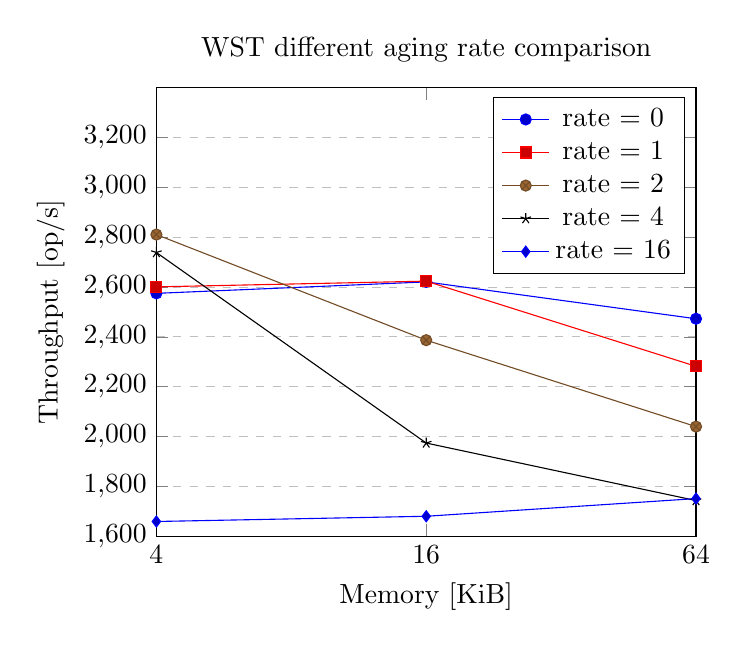
\begin{tikzpicture}
  \begin{axis}[
    title={\libname{WST} different aging rate comparison},
    xlabel = Memory {[KiB]},
    ylabel = Throughput {[op/s]},
    xmin = 1, xmax = 3,
    xtick={1,2,3},
    xticklabels={4, 16, 64},
    ymin = 1600, ymax = 3400,
    ytick={1600, 1800, 2000, 2200, 2400, 2600, 2800, 3000, 3200},
    ymajorgrids=true,
    grid style=dashed,
  ]
    \addplot coordinates{(1, 2575)(2, 2621)(3, 2473)};
    \addplot coordinates{(1, 2601)(2, 2624)(3, 2282)};
    \addplot coordinates{(1, 2811)(2, 2387)(3, 2040)};
    \addplot coordinates{(1, 2739)(2, 1974)(3, 1743)};
    \addplot coordinates{(1, 1659)(2, 1680)(3, 1751)};
    \legend{rate = 0, rate = 1, rate = 2, rate = 4, rate = 16}
  \end{axis}
  \end{tikzpicture}

  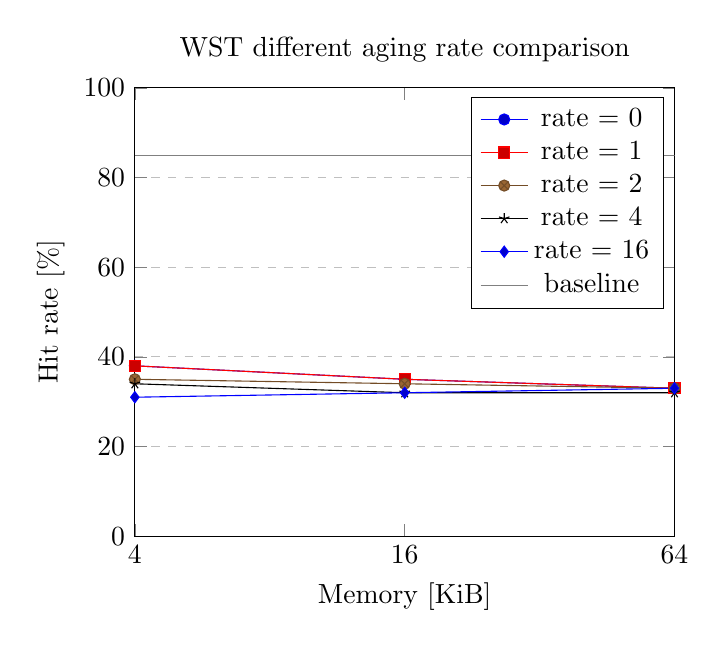
\begin{tikzpicture}
    \begin{axis}[
      title={\libname{WST} different aging rate comparison},
      xlabel = Memory {[KiB]},
      ylabel = Hit rate {[\%]},
      xmin = 1, xmax = 3,
      xtick={1,2,3},
      xticklabels={4, 16, 64},
      ymin = 0, ymax = 100,
      ymajorgrids=true,
      grid style=dashed,
    ]
      \addplot coordinates{(1, 38)(2, 35)(3, 33)};
      \addplot coordinates{(1, 38)(2, 35)(3, 33)};
      \addplot coordinates{(1, 35)(2, 34)(3, 33)};
      \addplot coordinates{(1, 34)(2, 32)(3, 32)};
      \addplot coordinates{(1, 31)(2, 32)(3, 33)};
      \addplot[color=gray] coordinates{(1, 85)(2, 85)(3, 85)};
      \legend{rate = 0, rate = 1, rate = 2, rate = 4, rate = 16, baseline}
    \end{axis}
    \end{tikzpicture}

    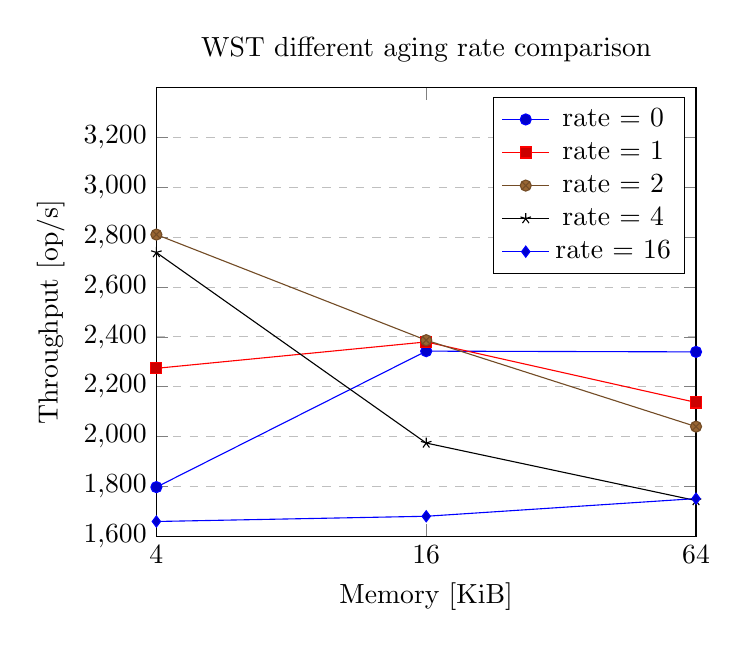
\begin{tikzpicture}
      \begin{axis}[
        title={\libname{WST} different aging rate comparison},
        xlabel = Memory {[KiB]},
        ylabel = Throughput {[op/s]},
        xmin = 1, xmax = 3,
        xtick={1,2,3},
        xticklabels={4, 16, 64},
        ymin = 1600, ymax = 3400,
        ytick={1600, 1800, 2000, 2200, 2400, 2600, 2800, 3000, 3200},
        ymajorgrids=true,
        grid style=dashed,
      ]
        \addplot coordinates{(1, 1797)(2, 2343)(3, 2340)};
        \addplot coordinates{(1, 2274)(2, 2380)(3, 2137)};
        \addplot coordinates{(1, 2811)(2, 2387)(3, 2040)};
        \addplot coordinates{(1, 2739)(2, 1974)(3, 1743)};
        \addplot coordinates{(1, 1659)(2, 1680)(3, 1751)};
        \legend{rate = 0, rate = 1, rate = 2, rate = 4, rate = 16}
      \end{axis}
      \end{tikzpicture}

      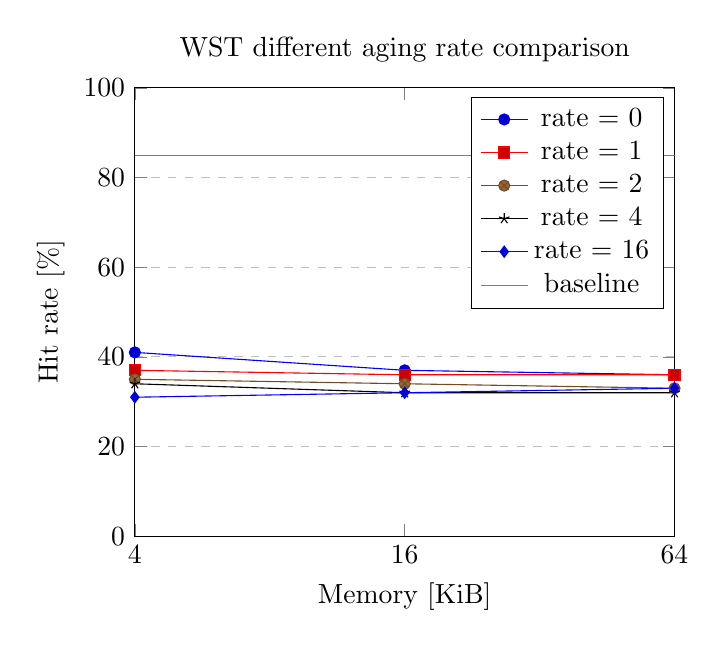
\begin{tikzpicture}
        \begin{axis}[
          title={\libname{WST} different aging rate comparison},
          xlabel = Memory {[KiB]},
          ylabel = Hit rate {[\%]},
          xmin = 1, xmax = 3,
          xtick={1,2,3},
          xticklabels={4, 16, 64},
          ymin = 0, ymax = 100,
          ymajorgrids=true,
          grid style=dashed,
        ]
          \addplot coordinates{(1, 41)(2, 37)(3, 36)};
          \addplot coordinates{(1, 37)(2, 36)(3, 36)};
          \addplot coordinates{(1, 35)(2, 34)(3, 33)};
          \addplot coordinates{(1, 34)(2, 32)(3, 32)};
          \addplot coordinates{(1, 31)(2, 32)(3, 33)};
          \addplot[color=gray] coordinates{(1, 85)(2, 85)(3, 85)};
          \legend{rate = 0, rate = 1, rate = 2, rate = 4, rate = 16, baseline}
        \end{axis}
        \end{tikzpicture}
\end{center}
